% ------------------------------------------------------------------------
% Relatório Técnico -- Projeto Final (Tema 04: Rede Social Simplificada)
% Estruturas de Dados -- UFU -- Prof.a Camila Davi Ramos -- 2026/1
%
% Classe: abnTeX2 (https://www.abntex.net.br/), em conformidade com as
% normas ABNT (NBR 14724 / NBR 10719) para relatórios técnico-acadêmicos.
%
% Compilação (após instalar texlive-latex-base, texlive-latex-recommended,
% texlive-latex-extra, texlive-lang-portuguese, texlive-fonts-recommended,
% texlive-publishers e texlive-pictures):
%
%   pdflatex relatorio.tex
%   pdflatex relatorio.tex   (rodar 2x para o sumario sair correto)
%
% ------------------------------------------------------------------------

\documentclass[
	12pt,				% tamanho da fonte
	oneside,			% documento digital: sem forçar capítulos em página ímpar
	a4paper,			% tamanho do papel
	chapter=TITLE,		% títulos de capítulo (seções primárias) em maiúsculas, conforme NBR 14724
	brazil,				% idioma principal do documento
	]{abntex2}

% ---
% Pacotes fundamentais
% ---
\usepackage{lmodern}
\usepackage[T1]{fontenc}
\usepackage[utf8]{inputenc}
\usepackage{indentfirst}
\usepackage{color}
\usepackage{graphicx}
\usepackage{microtype}
\usepackage{booktabs}
\usepackage{array}
\usepackage{amsmath}
\usepackage{tikz}
% ---

% ---
% Rede de segurança: define \legend apenas se a classe ainda não o fizer
% (comando do abnTeX2 para a linha "Fonte: ..." abaixo de figuras/tabelas).
% ---
\providecommand{\legend}[1]{\par\vspace{-0.4\baselineskip}{\footnotesize #1\par}\vspace{0.2cm}}

% ---
% Listagens (usadas para reproduzir capturas reais de execução do terminal)
% ---
\usepackage{listings}
\definecolor{corfundoterminal}{rgb}{0.94,0.94,0.94}
\lstdefinestyle{terminal}{
	basicstyle=\ttfamily\footnotesize,
	breaklines=true,
	frame=single,
	backgroundcolor=\color{corfundoterminal},
	columns=fullflexible,
	keepspaces=true,
	showstringspaces=false,
	breakindent=0pt,
	xleftmargin=2pt,
	xrightmargin=2pt
}
\lstset{style=terminal}

% ---
% Informações de dados para a CAPA
% ---
\titulo{Rede Social Simplificada}
\autor{%
	Débora Cristina Pereira Marra (12411ECP017) \and
	Gabriel Martins Santos Almeida (12411ECP012) \and
	Jose Lucas Lira Bizil (12411ECP005) \and
	Nycholas Rodrigues Cunha Coelho (12521ECP031) \and
	Vitor Augusto Machado Silami (12411ECP019)
}
\local{Uberlândia -- MG}
\data{Julho de 2026}
\instituicao{%
	Universidade Federal de Uberlândia -- UFU
	\par
	Faculdade de Engenharia Elétrica
	\par
	Disciplina de Estruturas de Dados}
\tipotrabalho{Relatório técnico -- Projeto Final (Tema 04)}
\preambulo{Relatório técnico referente ao Projeto Final (Tema 04 -- Rede
Social Simplificada) apresentado à disciplina de Estruturas de Dados da
Faculdade de Engenharia Elétrica da Universidade Federal de Uberlândia, sob
orientação da Profa. Camila Davi Ramos, como requisito parcial de avaliação
do semestre 2026/1.}
% ---

% ---
% Metadados do PDF
% ---
\makeatletter
\hypersetup{
	pdftitle={\@title},
	pdfauthor={\@author},
	pdfsubject={\imprimirpreambulo},
	pdfcreator={LaTeX com abnTeX2},
	pdfkeywords={estruturas de dados}{rede social}{C}{ABNT},
	colorlinks=true,
	linkcolor=black,
	citecolor=black,
	filecolor=black,
	urlcolor=blue,
	bookmarksdepth=3
}
\makeatother
% ---

% ---
% Espaçamentos
% ---
\setlength{\parindent}{1.3cm}
\setlength{\parskip}{0.2cm}

\begin{document}

\selectlanguage{brazil}
\frenchspacing

% ----------------------------------------------------------
% ELEMENTOS PRÉ-TEXTUAIS
% ----------------------------------------------------------
\pretextual

\imprimircapa

\pdfbookmark[0]{\contentsname}{toc}
\tableofcontents*
\clearpage

% ----------------------------------------------------------
% ELEMENTOS TEXTUAIS
% ----------------------------------------------------------
\textual

% ============================================================
\chapter{Introdução}
% ============================================================

Redes sociais digitais armazenam e relacionam grandes volumes de dados de
usuários, conexões e conteúdo publicado, exigindo estruturas de dados
capazes de sustentar operações de busca, inserção e travessia com
desempenho previsível à medida que a base de usuários cresce. Este
relatório descreve o desenvolvimento de uma \emph{rede social simplificada},
implementada em linguagem C, como Projeto Final da disciplina de Estruturas
de Dados (Tema 04), contemplando cadastro e busca de usuários, gestão de
amizades, publicações, histórico de atividades e sugestão de novas
conexões.

Um Tipo Abstrato de Dados (TAD) define um conjunto de dados e as operações
permitidas sobre eles, independentemente de sua implementação interna
(CORMEN et al., 2012). A escolha do TAD adequado a cada funcionalidade
determina diretamente a complexidade assintótica das operações do sistema,
normalmente expressa pela notação O(\emph{n}): O(1) para operações de custo
constante, O(log \emph{n}) para buscas em estruturas balanceadas e O(\emph{n})
para percursos lineares (ZIVIANI, 2011).

No sistema desenvolvido, seis TADs clássicos foram empregados, cada um
resolvendo um subproblema específico:

\begin{enumerate}
	\item uma \textbf{árvore binária de busca balanceada (AVL)} indexa os
	usuários pelo identificador (\emph{id}), garantindo busca em O(log
	\emph{n}) mesmo no pior caso;
	\item uma \textbf{tabela hash} com tratamento de colisões por
	encadeamento separado indexa os usuários por \emph{login} e por nome,
	com custo médio O(1), realocando (\emph{rehash}) seus baldes
	dinamicamente para preservar esse desempenho;
	\item uma \textbf{lista encadeada} genérica armazena as publicações de
	cada usuário e as listas de adjacência do grafo;
	\item uma \textbf{fila} (FIFO) sustenta a busca em largura (\emph{BFS})
	usada para verificar conectividade e gerar sugestões de amizade;
	\item uma \textbf{pilha} (LIFO) mantém o histórico das atividades mais
	recentes, sempre exibido da mais nova para a mais antiga;
	\item um \textbf{grafo} não direcionado representa a rede de amizades
	entre os usuários.
\end{enumerate}

O objetivo deste trabalho é apresentar o projeto, a modelagem e os
resultados obtidos na implementação de um sistema de rede social
simplificada em C, atendendo às dez funcionalidades obrigatórias e aos três
requisitos não funcionais especificados no enunciado do Projeto Final --
Tema 04, com ênfase na justificativa do uso correto e eficiente de cada
estrutura de dados exigida.

% ============================================================
\chapter{Métodos}
% ============================================================

\section{Arquitetura geral}

O sistema é organizado em módulos independentes, cada TAD implementado como
um par de arquivos \texttt{.h}/\texttt{.c}, conforme exigido no enunciado. O
arquivo \texttt{main.c} é responsável apenas pela interface de menu (E/S
com o usuário) e não contém regra de negócio; toda a lógica de cadastro,
validação e integração entre as estruturas está concentrada no módulo de
fachada \texttt{rede\_social}, que mantém a árvore AVL, as duas tabelas
hash, o grafo de amizades e a pilha de histórico, delegando a cada TAD
apenas a responsabilidade que lhe é própria. O módulo \texttt{persistencia}
lê e grava o estado da fachada em um arquivo de texto
(\texttt{rede\_social.dat}), sem que os demais módulos precisem conhecer o
formato de armazenamento. A Figura \ref{fig:arquitetura} ilustra essa
arquitetura.

\begin{figure}[htb]
\centering
\resizebox{\linewidth}{!}{%
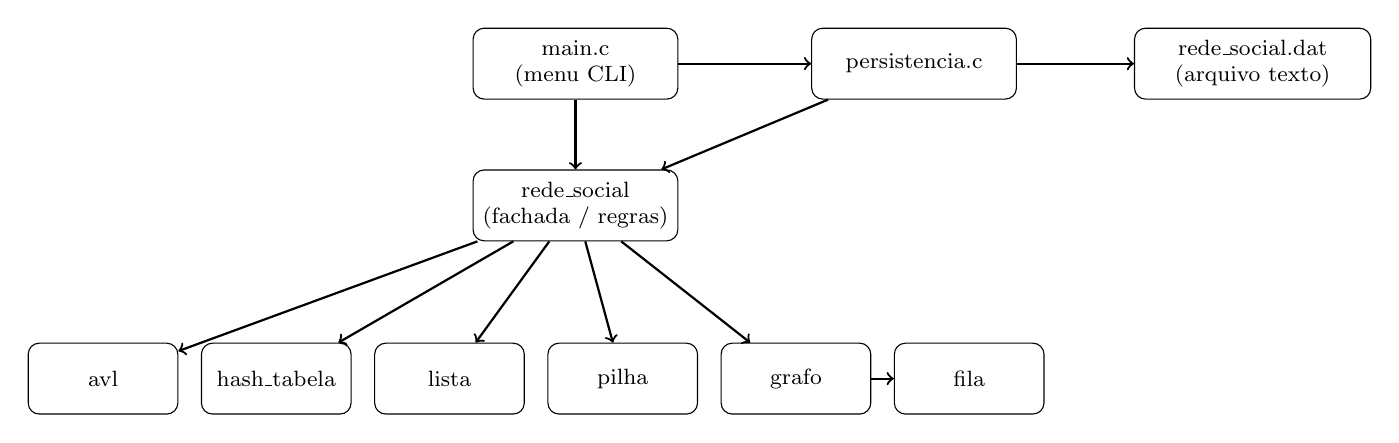
\begin{tikzpicture}[
	box/.style={draw, rectangle, rounded corners, minimum width=2.6cm, minimum height=0.9cm, align=center, font=\footnotesize},
	seta/.style={->, thick}
	]
	\node[box] (main) at (0,4) {main.c\\(menu CLI)};
	\node[box] (persist) at (4.3,4) {persistencia.c};
	\node[box, minimum width=3.0cm] (dat) at (8.6,4) {rede\_social.dat\\(arquivo texto)};
	\node[box] (fachada) at (0,2.2) {rede\_social\\(fachada / regras)};

	\node[box, minimum width=1.9cm] (avl) at (-6.0,0) {avl};
	\node[box, minimum width=1.9cm] (hash) at (-3.8,0) {hash\_tabela};
	\node[box, minimum width=1.9cm] (lista) at (-1.6,0) {lista};
	\node[box, minimum width=1.9cm] (pilha) at (0.6,0) {pilha};
	\node[box, minimum width=1.9cm] (grafo) at (2.8,0) {grafo};
	\node[box, minimum width=1.9cm] (fila) at (5.0,0) {fila};

	\draw[seta] (main) -- (fachada);
	\draw[seta] (main) -- (persist);
	\draw[seta] (persist) -- (dat);
	\draw[seta] (persist) -- (fachada);
	\draw[seta] (fachada) -- (avl);
	\draw[seta] (fachada) -- (hash);
	\draw[seta] (fachada) -- (lista);
	\draw[seta] (fachada) -- (pilha);
	\draw[seta] (fachada) -- (grafo);
	\draw[seta] (grafo) -- (fila);
\end{tikzpicture}%
}
\caption{Arquitetura de módulos do sistema}
\label{fig:arquitetura}
\legend{Fonte: elaborado pelos autores.}
\end{figure}

\section{Modelagem dos TADs}

\subsection{Árvore AVL (índice por id)}

A árvore AVL indexa cada \texttt{Usuario} pelo campo \texttt{id}, atribuído
automaticamente e de forma sequencial no cadastro. Cada nó armazena o
\emph{id}, um ponteiro para o usuário e sua altura, recalculada a cada
inserção; quando o fator de balanceamento de um nó ultrapassa 1 em módulo,
uma das quatro rotações clássicas (simples à esquerda, simples à direita,
dupla esquerda-direita ou dupla direita-esquerda) é aplicada. Como o
enunciado não exige remoção de usuários -- apenas de amizades --, a árvore
implementa somente inserção, busca e percurso em ordem (usado pela
persistência), o que simplifica a implementação sem abrir mão da garantia
de O(log \emph{n}) mesmo quando os \emph{ids} são inseridos em sequência
crescente, caso em que uma BST comum degeneraria em uma lista.

\subsection{Tabela hash (índice por login e por nome)}

Duas instâncias de uma mesma tabela hash genérica (chave textual $\to$
ponteiro) indexam os usuários: uma por \texttt{login}, chave única usada
para impedir cadastros duplicados, e outra por \texttt{nome}, que aceita
múltiplos usuários por chave (acumulados em uma lista encadeada) para
suportar a busca por nome. Colisões são tratadas por encadeamento separado
(Figura \ref{fig:hash}); a função de espalhamento utilizada é a
\emph{djb2}. Para preservar o custo médio O(1) mesmo com o crescimento da
base de usuários, a tabela dobra o número de baldes e redistribui todas as
entradas sempre que o fator de carga ultrapassa 0,75.

\begin{figure}[htb]
\centering
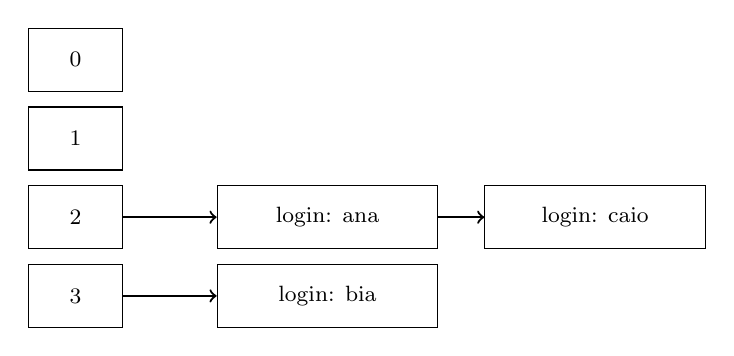
\begin{tikzpicture}[
	bkt/.style={draw, rectangle, minimum width=1.2cm, minimum height=0.8cm, font=\footnotesize},
	no/.style={draw, rectangle, minimum width=2.8cm, minimum height=0.8cm, font=\footnotesize, align=center},
	seta/.style={->, thick}
	]
	\node[bkt] (b0) at (0,3) {0};
	\node[bkt] (b1) at (0,2) {1};
	\node[bkt] (b2) at (0,1) {2};
	\node[bkt] (b3) at (0,0) {3};

	\node[no] (n2a) at (3.2,1) {login: ana};
	\node[no] (n2b) at (6.6,1) {login: caio};
	\node[no] (n3a) at (3.2,0) {login: bia};

	\draw[seta] (b2) -- (n2a);
	\draw[seta] (n2a) -- (n2b);
	\draw[seta] (b3) -- (n3a);
\end{tikzpicture}
\caption{Tabela hash com tratamento de colisões por encadeamento separado}
\label{fig:hash}
\legend{Fonte: elaborado pelos autores. Baldes 0 e 1 vazios; balde 2 com
colisão de duas chaves distintas.}
\end{figure}

\subsection{Lista, fila e pilha}

A lista encadeada é implementada de forma genérica (armazena
\texttt{void*}) e reaproveitada em dois papéis: como lista de publicações
de cada usuário -- inserção sempre no início, de modo que a publicação
mais recente apareça primeiro -- e como lista de adjacência do grafo de
amizades. A fila (FIFO) sustenta a busca em largura (\emph{BFS}) usada
tanto para verificar conectividade quanto para gerar sugestões de amizade.
A pilha (LIFO) registra o histórico das $N=10$ atividades mais recentes do
sistema (novo usuário, nova amizade, remoção de amizade e nova
publicação); ao ultrapassar essa capacidade, a atividade mais antiga é
descartada automaticamente, e o percurso do topo para a base entrega os
eventos da mais recente para a mais antiga, exatamente como pedido no
enunciado.

\subsection{Grafo de amizades}

O grafo de amizades é não direcionado e implementado de forma desacoplada
da \texttt{struct Usuario}: seus vértices são simplesmente os \emph{ids}
dos usuários, e cada vértice mantém uma lista de adjacência com os
\emph{ids} de seus amigos diretos. Essa independência permite que o grafo
seja testado isoladamente, sem depender de nenhuma outra estrutura do
sistema. Duas operações relevantes utilizam busca em largura (\emph{BFS}):
a \textbf{verificação de conexão} entre dois usuários, que percorre o
grafo a partir da origem até encontrar o destino ou esgotar os vértices
alcançáveis; e a \textbf{sugestão de amizades}, que identifica os vértices
a exatamente distância 2 da origem (amigos de amigos, excluindo os amigos
diretos e o próprio usuário), conta quantos amigos em comum cada candidato
tem com a origem e ordena o resultado por esse número de forma
decrescente, com empates desfeitos em ordem alfabética pelo nome --
limitando a saída a três sugestões, como exigido. A Figura
\ref{fig:grafo} ilustra o cenário usado no caso de teste de sugestão de
amizades (Seção \ref{sec:capturas}, item X).

\begin{figure}[htb]
\centering
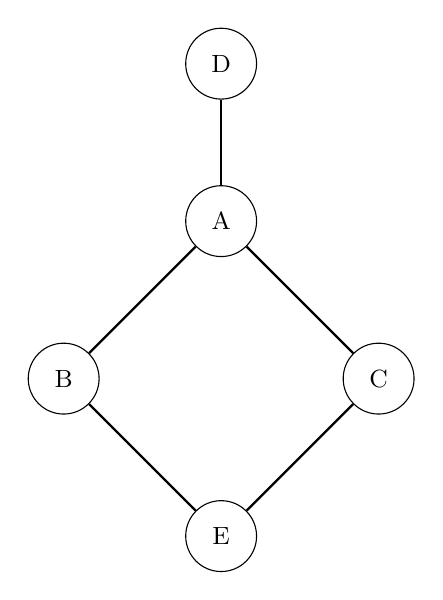
\begin{tikzpicture}[
	no/.style={draw, circle, minimum size=0.9cm, font=\small},
	seta/.style={thick}
	]
	\node[no] (A) at (0,2)  {A};
	\node[no] (B) at (-2,0) {B};
	\node[no] (C) at (2,0)  {C};
	\node[no] (D) at (0,4)  {D};
	\node[no] (E) at (0,-2) {E};

	\draw[seta] (A) -- (B);
	\draw[seta] (A) -- (C);
	\draw[seta] (A) -- (D);
	\draw[seta] (E) -- (B);
	\draw[seta] (E) -- (C);
\end{tikzpicture}
\caption{Exemplo de grafo de amizades usado no caso de teste de sugestão}
\label{fig:grafo}
\legend{Fonte: elaborado pelos autores. A busca em largura a partir de E
alcança A em profundidade 2 (via B e via C), tornando A a única sugestão,
com 2 amigos em comum.}
\end{figure}

% ============================================================
\chapter{Resultados}
% ============================================================

\section{Complexidade das operações}

A Tabela \ref{tab:complexidade-tad} resume a complexidade assintótica das
principais operações de cada TAD implementado, e a Tabela
\ref{tab:complexidade-func} mapeia essa complexidade para cada
funcionalidade obrigatória do enunciado. Em ambas, $n$ é o número de
usuários cadastrados, $V$ e $E$ são o número de vértices e arestas do
grafo de amizades, $N=10$ é o tamanho fixo do histórico e ``grau'' é o
número de amigos diretos de um usuário.

\begin{table}[htb]
\caption{Complexidade das operações por TAD}
\label{tab:complexidade-tad}
\centering
\begin{tabular}{
	>{\raggedright\arraybackslash}p{2.5cm}
	>{\raggedright\arraybackslash}p{3.0cm}
	>{\raggedright\arraybackslash}p{2.8cm}
	>{\raggedright\arraybackslash}p{5.0cm}}
\toprule
\textbf{Estrutura} & \textbf{Operação} & \textbf{Complexidade} & \textbf{Observação} \\
\midrule
Árvore AVL   & Inserir            & O(log $n$) & Balanceada; nunca degenera \\
Árvore AVL   & Buscar por id      & O(log $n$) & \\
Tabela hash  & Inserir / buscar   & O(1) médio & \emph{Rehash} ao superar fator de carga 0,75 \\
Lista        & Inserir (início/fim) & O(1) & Mantém ponteiros início/fim \\
Lista        & Buscar / remover valor & O($k$) & $k$ = tamanho da lista \\
Fila         & (Des)enfileirar    & O(1) & \\
Pilha        & Empilhar           & O(1) & Descarta o mais antigo se $> N$ \\
Pilha        & Percorrer histórico & O($N$) & $N=10$, constante \\
Grafo        & Adicionar/remover aresta & O(grau) & Verifica duplicidade antes \\
Grafo        & Verificar conexão (BFS) & O($V+E$) & \\
Grafo        & Sugerir amizades (BFS + contagem) & O($V+E+\text{grau}^2$) & Pior caso \\
\bottomrule
\end{tabular}
\legend{Fonte: elaborado pelos autores, a partir da implementação em \texttt{src/}.}
\end{table}

\begin{table}[htb]
\caption{Complexidade dominante por funcionalidade obrigatória}
\label{tab:complexidade-func}
\centering
\begin{tabular}{lll}
\toprule
\textbf{Funcionalidade} & \textbf{Estruturas envolvidas} & \textbf{Complexidade} \\
\midrule
I. Cadastro de usuário         & AVL + Hash (login/nome) + Grafo & O(log $n$) \\
II. Busca por nome              & Tabela hash (nome)              & O(1) médio + O($k$) \\
III. Adicionar amizade          & Grafo                           & O(grau) \\
IV. Remover amizade             & Grafo                           & O(grau) \\
V. Criar publicação             & AVL (localizar) + Lista         & O(log $n$) \\
VI. Exibir publicações          & Lista                           & O($k$) \\
VII. Histórico                  & Pilha                           & O($N$) \\
VIII. Exibir amigos             & Grafo + AVL                     & O(grau $\times$ log $n$) \\
IX. Verificar conexão           & Grafo (BFS)                     & O($V+E$) \\
X. Sugestão de amizades         & Grafo (BFS)                     & O($V+E+\text{grau}^2$) \\
\bottomrule
\end{tabular}
\legend{Fonte: elaborado pelos autores. $k$ representa o número de itens
retornados (amigos, publicações ou resultados de busca).}
\end{table}

\section{Capturas de execução dos casos de teste}
\label{sec:capturas}

Esta seção reproduz, para cada funcionalidade obrigatória, a saída real
obtida ao executar o binário \texttt{bin/\allowbreak rede\_social} com os
cenários descritos em \texttt{tests/\allowbreak casos\_teste.md}. As capturas abaixo são
transcrições literais do terminal (\emph{stdout}), não simulações.

\subsection{I. Cadastro de usuário}

\begin{lstlisting}
Opcao: 1
Nome: Ana Souza
Login: ana
Usuario cadastrado com sucesso! id = 1
\end{lstlisting}

Caso de erro (login duplicado):
\begin{lstlisting}
Opcao: 1
Nome: Outro Nome
Login: ana
Erro: Ja existe um usuario cadastrado com esse login.
\end{lstlisting}

\subsection{II. Busca de usuário por nome}

\begin{lstlisting}
Opcao: 2
Nome a buscar: Ana Souza
Usuarios encontrados:
  - id 1 | nome: Ana Souza | login: ana
\end{lstlisting}

Caso de erro (nome inexistente):
\begin{lstlisting}
Opcao: 2
Nome a buscar: Ninguem Assim
Nenhum usuario encontrado com o nome "Ninguem Assim".
\end{lstlisting}

\subsection{III. Adicionar amizade}

\begin{lstlisting}
Opcao: 3
Id do primeiro usuario: 1
Id do segundo usuario: 2
Amizade criada com sucesso.
\end{lstlisting}

Caso de erro (amizade duplicada):
\begin{lstlisting}
Opcao: 3
Id do primeiro usuario: 1
Id do segundo usuario: 2
Erro: Esses usuarios ja sao amigos.
\end{lstlisting}

\subsection{IV. Remover amizade}

\begin{lstlisting}
Opcao: 4
Id do primeiro usuario: 1
Id do segundo usuario: 2
Amizade removida com sucesso.
\end{lstlisting}

Caso de erro (remoção de amizade inexistente):
\begin{lstlisting}
Opcao: 4
Id do primeiro usuario: 1
Id do segundo usuario: 2
Erro: Esses usuarios nao sao amigos.
\end{lstlisting}

\subsection{V. Criar publicação}

\begin{lstlisting}
Opcao: 5
Id do usuario: 1
Texto da publicacao: Ola, mundo!
Publicacao criada com sucesso.
\end{lstlisting}

\subsection{VI. Exibir publicações}

\begin{lstlisting}
Opcao: 6
Id do usuario: 1
Publicacoes de Ana Souza (mais recente primeiro):
  - Ola, mundo!
\end{lstlisting}

\subsection{VII. Histórico (N=10, mais recente primeiro)}

\begin{lstlisting}
Opcao: 7
Historico de atividades (mais recente primeiro):
  [Nova publicacao] Nova publicacao de Ana Souza (id 1)
  [Nova amizade] Nova amizade: Ana Souza (id 1) e Carla Dias (id 3)
  [Nova amizade] Nova amizade: Ana Souza (id 1) e Bruno Lima (id 2)
  [Novo usuario] Novo usuario cadastrado: Carla Dias (id 3, login carla)
  [Novo usuario] Novo usuario cadastrado: Bruno Lima (id 2, login bruno)
  [Novo usuario] Novo usuario cadastrado: Ana Souza (id 1, login ana)
\end{lstlisting}

\subsection{VIII. Exibir amigos}

\begin{lstlisting}
Opcao: 8
Id do usuario: 1
Amigos de Ana Souza:
  - id 2 | nome: Bruno Lima | login: bruno
  - id 3 | nome: Carla Dias | login: carla
\end{lstlisting}

\subsection{IX. Verificar conexão entre usuários}

\begin{lstlisting}
Opcao: 9
Id do primeiro usuario: 1
Id do segundo usuario: 2
Os usuarios 1 e 2 estao conectados na rede.
\end{lstlisting}

\subsection{X. Sugestão de amizades}

\begin{lstlisting}
Opcao: 10
Id do usuario: 3
Sugestoes de amizade para Carla Dias:
  - Bruno Lima (id 2) | 1 amigo(s) em comum
\end{lstlisting}

\subsection{Requisito não funcional I: persistência}

O script \texttt{tests/\allowbreak smoke\_test.sh} automatiza a verificação deste
requisito: executa o binário três vezes em sequência, em um diretório
isolado, cadastrando usuários, amizade e publicação na primeira execução e
confirmando -- via busca por nome, exibição de amigos e exibição de
publicações -- que todos os dados persistiram nas execuções seguintes,
inclusive que o próximo \emph{id} gerado continua a sequência anterior (não
reinicia em 1). A execução real do script produz:

\begin{lstlisting}
Smoke test de persistencia: OK (3 execucoes sucessivas, dados preservados)
\end{lstlisting}

\subsection{Requisitos não funcionais II e III: validação e duplicidade}

Todas as funcionalidades tratam entradas inválidas ou inexistentes sem
encerrar o programa abruptamente -- ver os casos de erro já reproduzidos
nas Seções 3.2.1 a 3.2.4 e 3.2.9 (login duplicado, nome sem resultado,
amizade duplicada, remoção de amizade inexistente e ids inexistentes). Além
disso, entradas não numéricas no menu (letras, linhas vazias) são
detectadas e o usuário é solicitado a digitar novamente, como mostrado
abaixo:

\begin{lstlisting}
Opcao: abc
Entrada invalida. Digite um numero inteiro.
Opcao:
\end{lstlisting}

Essas verificações também são cobertas de forma automatizada em
\texttt{tests/\allowbreak test\_rede\_social.c} (fachada) e nos testes unitários de
cada TAD, totalizando 90 asserções executadas via \texttt{make test}, todas
aprovadas, com compilação limpa (\texttt{gcc -Wall -Wextra -std=c11}) e sem
nenhum aviso do compilador.

% ----------------------------------------------------------
% ELEMENTOS PÓS-TEXTUAIS
% ----------------------------------------------------------
\postextual

\chapter*{Referências}
\addcontentsline{toc}{chapter}{Referências}

\noindent
CORMEN, Thomas H. et al. \textbf{Algoritmos}: teoria e prática. 3. ed. Rio
de Janeiro: Elsevier, 2012.

\noindent
ZIVIANI, Nivio. \textbf{Projeto de algoritmos}: com implementações em
Pascal e C. 3. ed. São Paulo: Cengage Learning, 2011.

\end{document}
